\section{Actividad 01: Importación de datos usando el Wizard - SQL MANAGMENT.} 

1. Primeramente crearemos una base de datos llamada BDTEST\\
	\begin{center}
	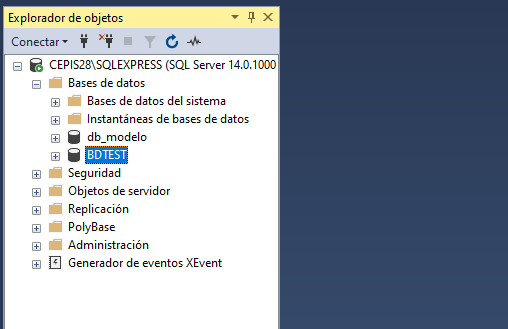
\includegraphics[width=11cm]{./Imagenes/img1}
	\end{center}	


2. Ahora importaremos nuestra base de datos desde AdventureWorks.\\
	\begin{center}
	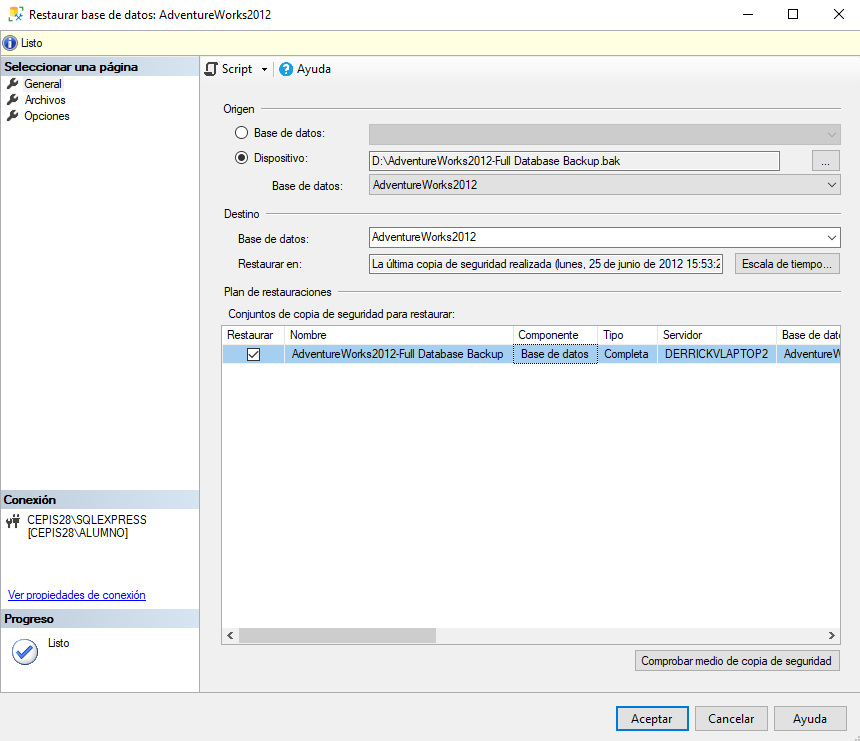
\includegraphics[width=11cm]{./Imagenes/img2}
	\end{center}	
\pagebreak
3. Next y escribir el Servidor y seleccionar la base de datos\\
	\begin{center}
	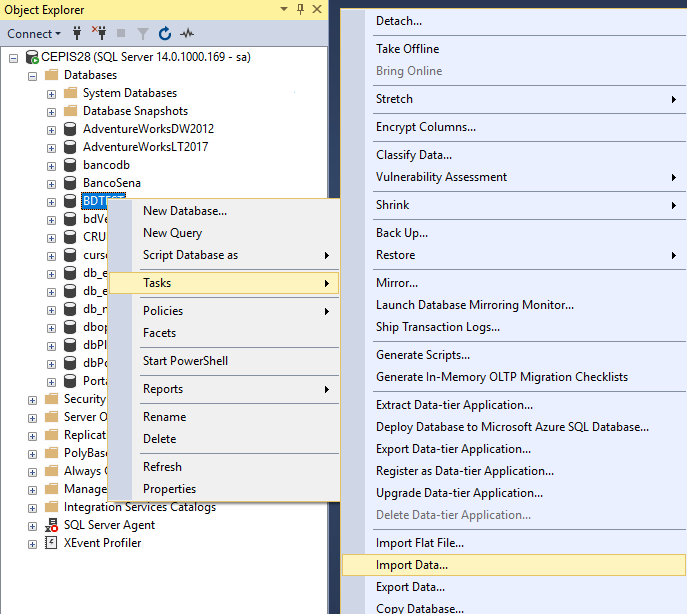
\includegraphics[width=11cm]{./Imagenes/img3}
	\end{center}	

4. Data Source: La base de donde vamos a importar - Destination: La Base donde vamos a cargar la datas\\
	\begin{center}
	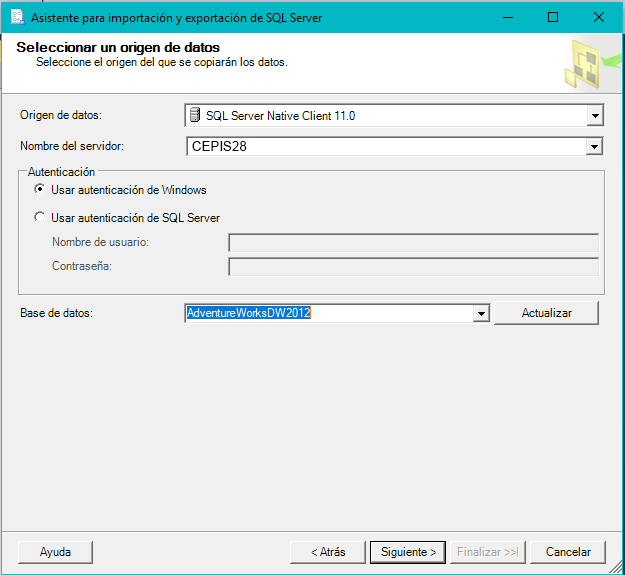
\includegraphics[width=11cm]{./Imagenes/img4}
	\end{center}	
	\begin{center}
	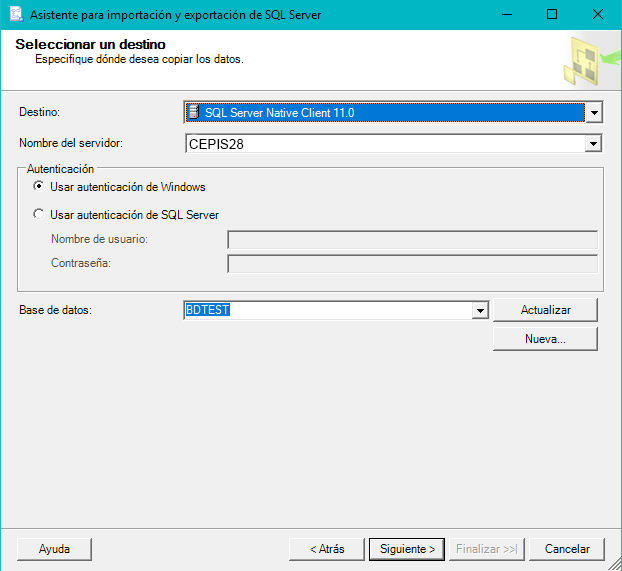
\includegraphics[width=11cm]{./Imagenes/img5}
	\end{center}	
	\begin{center}
	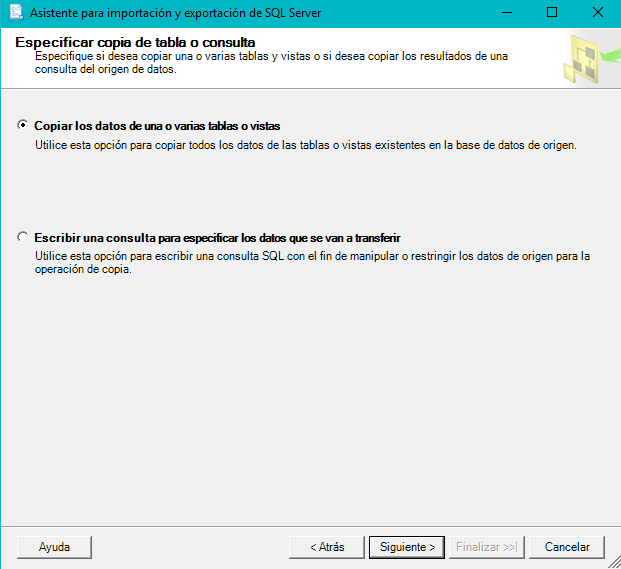
\includegraphics[width=11cm]{./Imagenes/img6}
	\end{center}	
	\begin{center}
	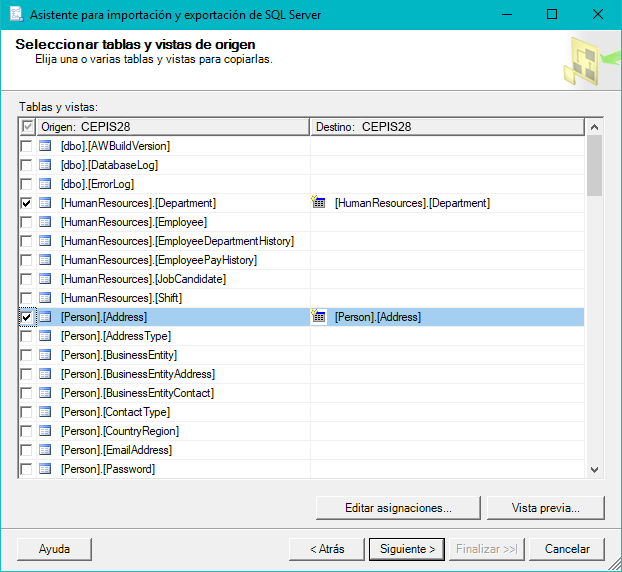
\includegraphics[width=11cm]{./Imagenes/img7}
	\end{center}	
	\begin{center}
	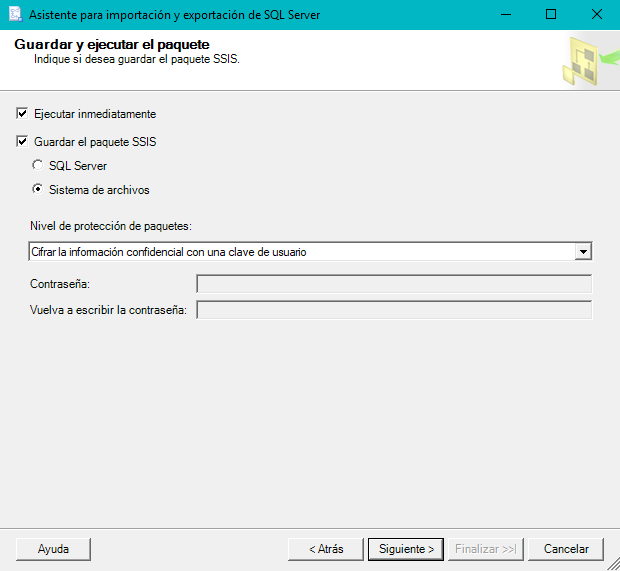
\includegraphics[width=11cm]{./Imagenes/img8}
	\end{center}	
	\begin{center}
	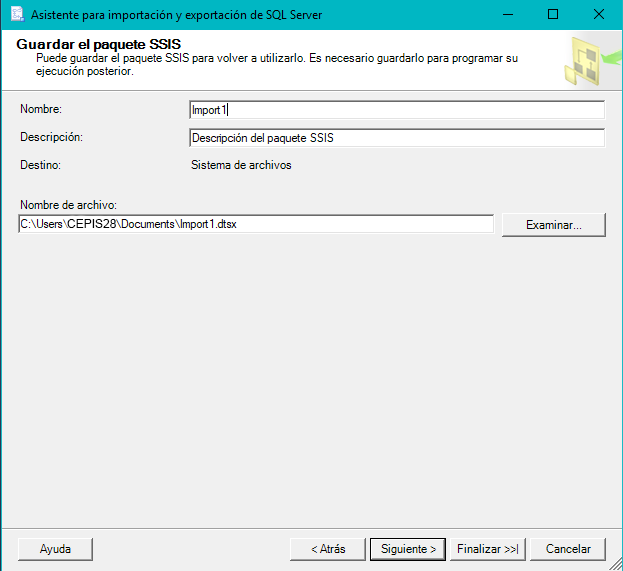
\includegraphics[width=11cm]{./Imagenes/img9}
	\end{center}	
	\begin{center}
	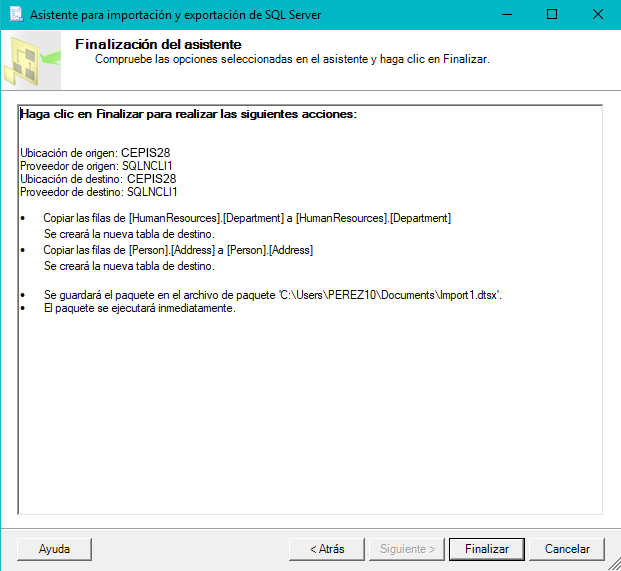
\includegraphics[width=11cm]{./Imagenes/img10}
	\end{center}	
	\begin{center}
	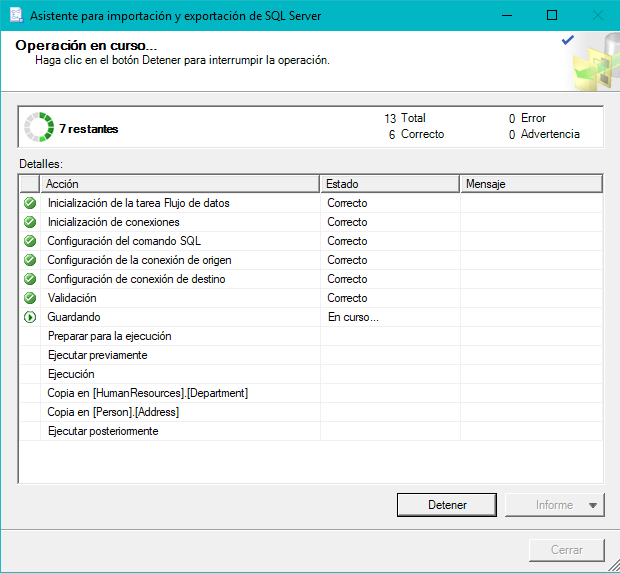
\includegraphics[width=11cm]{./Imagenes/img11}
	\end{center}	
5. Al final veremos un resumen de la ejecución\\
	\begin{center}
	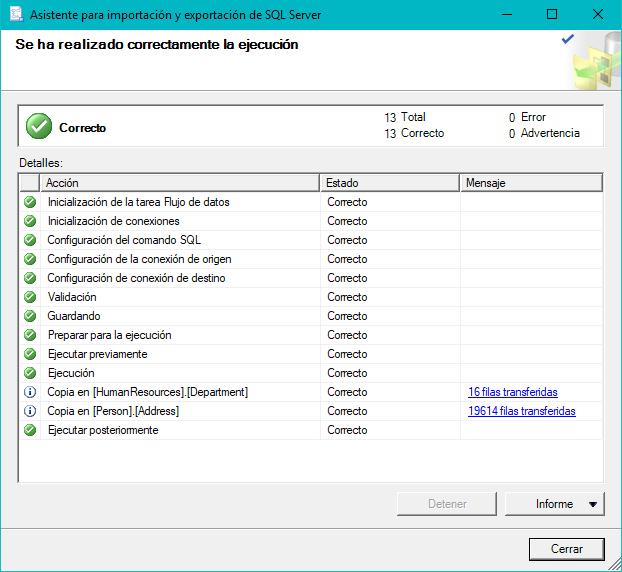
\includegraphics[width=11cm]{./Imagenes/img12}
	\end{center}	